\documentclass[a4paper,11pt,twoside,onecolumn,final,openright]{book}
\usepackage[doublespace,indent]{thesisdavid}
\usepackage[latin1]{inputenc}
\usepackage{subfigure}

\usepackage[english]{babel}
\usepackage{url}
\usepackage{epsfig}
\usepackage{epstopdf}
\usepackage{makeidx}
\usepackage{multirow}
\usepackage{indentfirst}
\usepackage[font=normalsize]{caption}
\usepackage{colortbl}
\usepackage{adjustbox}
\usepackage{enumitem}
\usepackage{graphicx}
\usepackage{array,booktabs,arydshln}
%\usepackage{rotating}
\usepackage{hyphenat}

\usepackage{xspace}
\usepackage{stfloats}
\usepackage{flushend}
\usepackage{listings}
\usepackage{color}
\usepackage[printonlyused]{acronym}


\definecolor{gray}{rgb}{0.4,0.4,0.4}
\definecolor{darkblue}{rgb}{0.0,0.0,0.6}
\definecolor{cyan}{rgb}{0.0,0.6,0.6}

\lstset{
  basicstyle=\ttfamily,
  columns=fullflexible,
  showstringspaces=false,
  commentstyle=\color{gray}\upshape
}

\definecolor{dkgreen}{rgb}{0,0.6,0}
\definecolor{gray}{rgb}{0.5,0.5,0.5}
\definecolor{mauve}{rgb}{0.58,0,0.82}
\lstset{frame=tb,
  language=Java,
  aboveskip=3mm,
  belowskip=3mm,
  showstringspaces=false,
  columns=flexible,
  basicstyle={\small\ttfamily},
  numbers=none,
  numberstyle=\tiny\color{gray},
  keywordstyle=\color{blue},
  commentstyle=\color{dkgreen},
  stringstyle=\color{mauve},
  breaklines=true,
  breakatwhitespace=true,
  tabsize=3
}

\lstdefinelanguage{XML}
{
  morestring=[b]",
  morestring=[s]{>}{<},
  morecomment=[s]{<?}{?>},
  stringstyle=\color{black},
  identifierstyle=\color{darkblue},
  keywordstyle=\color{cyan},
  morekeywords={xmlns,version,type}% list your attributes here
}

\newcolumntype{M}[1]{>{\centering\arraybackslash}m{#1}}

\newcommand{\red}[1]{\textcolor{red}{#1}}
\newcommand{\todo}[1]{\textcolor{red}{\{TODO:} #1\textcolor{red}\}}

\definecolor{light}{gray}{.85}

\begin{document}

% Initial pages.


\def\date{October 2015}
\def\titulo{SleeveAR: Augmented Reality for Rehabilitation Using Realtime Feedback}
\def\avitima{Jo\~{a}o Tiago Proen\c{c}a F\'elix Vieira}

\thispagestyle{empty}

\begin{singlespace}
\vbox to\textheight{%
%--------------------------------------------------
\vskip-1.3in%---------- LOGO E NOME IST/UTL -------
%--------------------------------------------------
\hskip-17mm\vbox to50mm{
\vfil
\begin{tabular}{l}

\includegraphics[width=9cm]{imgs/Logo_IST_web.pdf}
\end{tabular}
\vfil
\vfil
}%
%--------------------------------------------------
\vskip6mm%---------- TTULO -----------------------
%--------------------------------------------------
\vbox to25mm{\LARGE\bf
\vfil
\begin{center}
\titulo
\end{center}
\vfil
}%
%--------------------------------------------------
\vskip10mm%---------- NOME E GRAU ACTUAL -----------
%--------------------------------------------------
\vbox to25mm{\large
\vfil
\begin{center}
{\Large\bf \avitima}\\   % author's name
\end{center}
\vfil
}%
%--------------------------------------------------
\vskip10mm%---------- GRAU A OBTER -----------------

%--------------------------------------------------
\vbox to8mm{\large
\vfil
\centerline{Dissertation for the Degree of Master of}
%\vskip6mm
\centerline{Engineering Systems and Computer Engineering}
\vfil
}%
% %--------------------------------------------------
\vskip10mm %---------- JURI -------------------------
% %--------------------------------------------------
\vbox to7mm{\bf
\vfil
\begin{center}
{\bf Jury}\\
\end{center}
\vfil
}%

\vbox to28mm{
\vfil
{\small
\begin{center}
\begin{tabular}{p{0.2\textwidth}l}
President: &  PERGUNTAR AO ORIENTADOR \\
Advisor: & Prof. Joaquim Jorge\\
Co-Advisor: & Prof. Artur Ars\'enio\\
Member: & PERGUNTAR AO ORIENTADOR \\
\end{tabular}
\end{center}
}
\vfil
}%
%--------------------------------------------------
\vskip28mm%---------- DATA -------------------------
%--------------------------------------------------
\vbox to4mm{\Large\bf
\vfil
\begin{center}
\date
\end{center}
\vfil
}%
%--------------------------------------------------
}%vbox
\end{singlespace}
\newpage

\chapter*{Acknowledgements}
%\chapter*{Acknowledgements}
\thispagestyle{empty}

I would like to thank my canary.
Ana Paula Morais Cabral fisioterapeuta


\vfill
\begin{flushright}
  \begin{minipage}{8cm}
    \begin{center}
      Lisboa, \date

      \avitima
    \end{center}
  \end{minipage}
\end{flushright}

\cleardoublepage

  %%%%%%%%%%%%%%%%%%%%%%%%%%%%%%%%%%%%%%%%%%%%%%%%%%%%%%%%%%%%%%%%%%%%%%%%%%%%%
  %
%%%%%                            DEDICATORIAS
 %%%
  %

\chapter*{}
\thispagestyle{empty}

% DEDICAR!
\vfill
\mbox{}
\vfill\Large
\begin{flushright}
  \begin{minipage}{8cm}
    \begin{center}

For blablablablabla,\\

    \end{center}
  \end{minipage}
\end{flushright}
\normalsize\vfill

\cleardoublepage

  %%%%%%%%%%%%%%%%%%%%%%%%%%%%%%%%%%%%%%%%%%%%%%%%%%%%%%%%%%%%%%%%%%%%%%%%%%%%%
  %
%%%%%                                RESUMO
 %%%
  %

\chapter*{Resumo}
\thispagestyle{empty}
 
My abstract in Portuguese.

\newpage

  %%%%%%%%%%%%%%%%%%%%%%%%%%%%%%%%%%%%%%%%%%%%%%%%%%%%%%%%%%%%%%%%%%%%%%%%%%%%%
  %
%%%%%                            ABSTRACT
 %%%
  %

\chapter*{Abstract}
\thispagestyle{empty}

After being exempted from in-clinic physical therapy, 
	it is usual for a patient to continue performing exercises 
	outside of the clinic and without any therapist's supervision.
	While performing unsupervised exercises, it would be desirable 
	to receive similar feedback as the one provided by a physical therapist, to maintain 
	a certain quality in the task execution.
	To address this problem, several approaches using feedback for rehabilitation have been implemented. Unfortunately, the test subjects frequently reported difficulty in completely understanding the feedback given to them, therefore failing to correctly execute the given movement.

\newpage


\chapter*{Palavras Chave \\ Keywords}
\thispagestyle{empty}

\section*{Palavras Chave}
{\large % EM PORTUGUES

\noindent xxx

\noindent xxx

\noindent xxx

\noindent xxx

\noindent xxx

}

\section*{Keywords}

{\large % EM INGLES

\noindent xxx

\noindent xxx

\noindent xxx

\noindent xxx

\noindent xxx

}

\vfill


\cleardoublepage

\pagestyle{plain}
\pagenumbering{roman}

 
\def\contentsname{Contents}
\tableofcontents
\newpage

\listoffigures
\newpage

\listoftables

\cleardoublepage

       


\chapter*{Acronyms}

\begin{singlespace}

\begin{acronym}
	\acro{AR}{Augmented Reality}
	\acro{PT}{Physical Therapist}
	\acro{RS}{Rehabilitation System}
	\acro{KP}{Knowledge of Performance}
	\acro{KR}{Knowledge of Results}
	\acro{MFM}{Multimodal Feedback Manager}
	\acro{DTW}{Dynamic Time Warping}
	\acro{FS}{Feedback Service}
	\acro{ES}{Exercise Service}
	\acro{PP}{Physical Position}
	\acro{VP}{Virtual Position}
	\acro{PrP}{Projection Position}
\end{acronym}

\end{singlespace}


\pagenumbering{arabic}
\pagestyle{headings}

%%%%%%%%%%%%%%%%%%%%%%%%%%%%%%%%%%%%%%%%%%%%%%%%%%%%%%%%%%%%%%%%%%%%%%%%%%%%%%%%%%%%%%%%%%%
%                               Introduction - 3pp
%%%%%%%%%%%%%%%%%%%%%%%%%%%%%%%%%%%%%%%%%%%%%%%%%%%%%%%%%%%%%%%%%%%%%%%%%%%%%%%%%%%%%%%%%%%
\chapter{Introduction}
\label{sec:intro}

\section*{Summary}

\section{Motivation}


Even though physical therapy holds a great part of a injured person's rehabilitation, 
it also requires effort from the patient to achieve a full recovery.
In fact, the patient holds great responsibility in each therapy session.
He must be ready to learn about his condition and what types of therapeutic exercises 
to do and how to perform them whenever not being supervised by a therapist (e.g., whenever performing exercises at home).
To be able to exercise alone, a patient must be taught about his body and body 
movements, i.e., he must gain \emph{body awareness}.

A person with an acceptable body awareness has a better knowledge of his body and how to correctly move it when doing exercises or other tasks that involve physical movement.
Therefore, a person is able to improve the overall quality of a given movement and to diminish unnecessary muscle tension, 
by being able to use just the muscles required to accomplish a given task~\cite{Singh2014a}.
With relatively low body awareness, it becomes hard for a patient to perform well alone and may 
end up hurting himself. %arranjar exemplos?
Consequently, to help people with low awareness 
execute \textit{prescribed} tasks, it is necessary for them to receive real-time feedback.
This feedback is usually given by a professional, 
but without their presence, it would be desirable for people to receive similar feedback from other sources to maintain a certain quality in the task execution.

\ac{AR} is a technique used to impose digital content on top of the physical world, giving the user a different perception on the subject in which \ac{AR} is being applied. 
This can manipulate the meaning or increase the amount of information available of the subject being augmented.

\ac{AR} could be a possible solution to overpass the lack of clear feedback sources when no \ac{PT} is present.
It holds great potential in the field of rehabilitation %(and several other serious matters) 
and there are already a variety of tools available to help with the development process of Augmented
Reality applications that interact with the body~\cite{Gama2012a}.

If combined with a carefully designed form of feedback for the patient,
\ac{AR} can be of great use in the rehabilitation of a person ~\cite{Sigrist2013}. 
The whole idea of it is to give more information to a person in a way that it can make the assigned task easier to do.
Therefore, the type of feedback given by the \ac{AR} system can have a great influence 
on the outcome of the task being done~\cite{Causo2011}.

As above mentioned, the feedback given to a patient helps him to correct mistakes on the performed movements.
Usually, this feedback is given by a therapist while enduring physical therapy, which can be of a visual form (the therapist demonstrating what to do), auditory form (the therapist giving orders to the patient) or physical (the therapist applying physical force to the patient). 
When performing exercises alone, a different approach must be followed on the types of feedback used, making sure that the goals 
are still achieved and the patient performs the exercises correctly.

There are multiple types of feedback, just as there are forms of expression, which means that 
there could be different combinations of feedback that could make a patient understand the task better.
Most of the traditional feedback systems, used for rehabilitation, only use a singular type of feedback,
visual or auditory~\cite{Design2005}, being these kind of systems known as \emph{unimodal feedback systems}.

By using multiple types of feedback, we can take advantage of more than one sense on the patient, 
making it possible to give more information without overloading just one sense (e.g., just using visual
cues on a screen can become overwhelming for a patient). A system like the one described is called a 
\emph{multimodal feedback system}, which, by definition, uses various sensory inputs and outputs to achieve the desired task.

\section{Research Statement}

In this work, we introduce SleeveAR, a novel approach that provides awareness feedback to aid and guide the patient during rehabilitation exercises.
SleeveAR aims on providing the means for patients to precisely replicate the exercises, especially prescribed for them by a health professional. 
Since, the rehabilitation process relies on repetition of the exercises during the physiotherapy sessions, our approach contributes to the correct performance of the therapeutic exercises while offering reports on the patient's progress. 
Also, without rendering the role of the therapist obsolete, our approach builds on the notion that with proper guidance, the patients can execute rehabilitation exercises for themselves without full time supervision. 

With this dissertation, we intend to validate the assumption that using interactive applications relying on augmented reality and real-time feedback can become a better alternative to guide patients though rehabilitation without supervision, as oppose to other sources such as video observation. We can then highlight the research statement of this dissertation as follow:


\begin{quotation}
%\noindent \textit {\textbf {Is it possible to provide a level of awareness of remote people to the point that they are able to use proximity relationships in the development of collaborative tasks?}}
\noindent \textit {\textbf { SleeveAR can help patients exercise upper limb movements with greater efficiency to that of a unsupervised rehabilitation.}}

\end{quotation}


\section{Contributions}

With the development of our SleeveAR prototype, our work provides the following contributions:

\begin{itemize}
\item \textbf{Solution for unsupervised upper-limb rehabilitation}\\
The prototype developed in our work can help patients replicate rehabilitation exercises even if they did not observed the exercise prior to their execution.

\item \textbf{Content projection on moving surfaces}\\
We present a novel technique for projecting content on top of tracked objects. With this technique, we are able to provide visual feedback on the actual upper-limb being rehabilitated.

\item \textbf{New visual feedback designs}\\
We created a group of minimalist visual cues to guide patients which cover the majority of possible arm movements.

\end{itemize}
 

\section{Publications}


The work developed in this dissertation led to a publication evaluated by an international panel of experts and accepted in a scientific conferences. The publication is listed below.

\begin{enumerate}
\item \textit{Augmented Reality for Rehabilitation Using Multimodal Feedback}, \textbf{Jo\~{a}o Vieira}, Maur\'icio Sousa, Artur Ars\'enio and Joaquim Jorge, 3rd Workshop on ICTs for improving Patients Rehabilitation Research Techniques (REHAB 2015), October 2015.
\end{enumerate}


\section{Dissertation Outline}

The remaining content of this dissertation are organised as follows. 
In Chapter~\ref{section-related} we discuss related work that had influence on our approach, several state of the art works are presented and a comparison between them can be found. 
Chapter~\ref{sec:sleevear} introduces our proposed solution, SleeveAR. An approach on guiding patients through pre-recorded exercises with real-time correction feedback.
Next, in Chapter~\ref{sec:implementation}, we present our SleeveAR implementation, describing all the technology and development that allowed us to achieve our solution.
Chapter~\ref{sec:evaluation} reports the user tests conducted to evaluate our solution. 
And finally, in Chapter~\ref{sec:conclusions}, we present our conclusions and discuss our future work with SleeveAr.
%%%%%%%%%%%%%%%%%%%%%%%%%%%%%%%%%%%%%%%%%%%%%%%%%%%%%%%%%%%%%%%%%%%%%%%%%%%%%%%%%%%%%%%%%%%
%                               Related Work - 24-32pp
%%%%%%%%%%%%%%%%%%%%%%%%%%%%%%%%%%%%%%%%%%%%%%%%%%%%%%%%%%%%%%%%%%%%%%%%%%%%%%%%%%%%%%%%%%%
\chapter{Related Work}
\label{section-related}

\section*{Summary}

Motor rehabilitation, or motor re-learning, is an extensive and demanding process for a patient.
For a successful recovery, the patient must be disciplined and understand that this is a tough and painful task in which it
will normally be required to move the injured area which might cause immense pain\cite{Singh2014a}.
Depending on the injury, it requires several physical therapy sessions and, after finishing them, 
the rehabilitation might have to continue at the patient's own home\cite{Lohse2013}.

Home rehabilitation is common among injured individuals, since
attending sessions at a professional clinic is usually not enough for a full recovery.
The patient will need to add more effort outside of the clinic and continue 
exercising to avoid suffering a setback on his rehabilitation \cite{Borghese2013} 
or to increase his recovery speed. 
This requires him to learn what exercises to do and how to do 
them correctly to prevent an aggravation of the injury\cite{Tang2014a}.

There is a significant difference between rehabilitation with a \ac{PT} and without him.
When a patient is attending physical therapy, it is the therapist 
job to help him fight his pain and recover from his injury.
His role is fundamental to plan what exercises the patient must do and to make sure they are executed correctly. 
Since the patient does not always has the ability to execute alone the exercises, or not even move without an external help,
the therapist can intervene during the session and adapt his approach according to the patient's needs\cite{Sigrist2013}.
However, whenever the rehabilitation exercises are done at home, without the therapist presence, the patient might 
perform incorrect movements to avoid pain\cite{Tang2014a} or might not even be able to move at all.


Repeating specific movements is a key factor in motor re-learning \cite{Schonauer2011a} and it 
will always be a part of the rehabilitation, whether at a clinic or at home.
This is one of the main causes of deteriorated rehabilitation at home. In this case, patients tend to get bored and lose focus, 
due to this repetition and lack of a therapist presence to guide and motivate him \cite{Singh2014a,Balaam2011a,Rego2010}. 
To help with this unsupervised rehabilitation work, several solutions have appeared as 
an alternative to the classic paper or video instructions. 

Using modern technologies and counting on an increasing offer in 
affordable tracking devices (e.g. Microsoft Kinect), a large
diversity of applications are being developed that aim to solve 
some of the difficulties in unsupervised rehabilitation \cite{Kitsunezaki2013,Borghese2013}. Several such works, focused on rehabilitation, will be discussed in the next section.


\section{Rehabilitation Systems}

Nowadays, we can observe a wide variety of rehabilitation systems which can help improve the recovery of a patient. 
Many of them have different rehabilitation goals and focus on specific injuries, e.g., stroke\cite{Borghese2013,Design2005}, 
or limbs rehabilitation \cite{Sadihov2013,Burke2009,Klein2013}.

The use of these systems can have a great influence in a patient's rehabilitation outside of a clinic. 
Not only it allows to maintain a certain quality on the execution of exercises, but also enables 
the patient to exercise in a comfortable environment, his home, which makes it easier to stimulate 
and motivate him during the whole process \cite{Borghese2013}.

As it has been said previously, a patient's rehabilitation is related to three concepts: repetition, feedback and motivation \cite{Schonauer2011a}. 
Hence, the development of a \ac{RS} should always be influenced by these three ideas and how to approach them. 

The repetitive nature of rehabilitation exercises can quickly become boring for a patient\cite{Rego2010,Burke2009,Burdea2002}, 
therefore, there is a need of turning these exercises into something less tedious. 
It is believed that when dealing with repetitive exercises, the main goal should be divided into several sub-goals. This way the 
patient keeps achieving incremental success through each repetition and increases his motivation when comparing to the approach where success is only achieved after finishing the whole task \cite{Schonauer2011a}.

For a patient to be informed about his execution, the feedback provided can be given in two different ways. During the execution
(concurrent feedback) or at the end (terminal feedback)\cite{Sigrist2013}.
The concurrent feedback is given in real-time with the purpose of offering correction or guidance, 
it allows the patient to have \ac{KP}. On the other hand, terminal feedback only allows the patient 
to know if he succeeded after fully executing the task, giving him \ac{KR} \cite{Design2005, Schonauer2011a}. 

Studies have shown a difficulty in obtaining a flawless formula when it comes to relating \ac{KP} and \ac{KR}. 
On one hand, \ac{KP} helps to accelerate the learning process of the exercise by correcting the patient in
real-time. On the other hand, prolonged \ac{KP} can create a dependency on the feedback, interfering with the 
learning process. Therefore, Sigrist \cite{Sigrist2013} states that \ac{KP} should be reduced as the exercise
keeps advancing, gradually giving more emphasis to \ac{KR} in order to stimulate the autonomy of the patient.

Gama et al. \cite{Gama2012a} developed a rehabilitation system in which the user position was tracked using a 
Microsoft Kinect. In this system, the user would see himself on the screen with overlaying targets that represented the desired position. 
If a incorrect posture was detected (shoulders not aligned or arm not fully stretched) he would be notified in real-time with visual messages. 
White arrows on the screen were also used as visual cues to guide the patient's arm to the target.
For each repetition, points were added to a score, depending on how well the user performed.
%\todo{conclusao} \todo{falar de knowledge of performance/result em separado para cada referencia?}
%In this paper we can notice the use of \ac{KP} with 

Another work \cite{Klein2013} focused on rehabilitating stroke victims which normally end up with one of the arms extremely debilitated.
In this case, the main focus was to motivate the patient to move his injured arm. Even with a small range of motion, it is 
important for the patient to move it in order to improve the recovery. The patient would see a virtual arm overlaying his injured arm, which would simulate a normal arm movement. 
The virtual arm position was calculated based on a few control points around the patients shoulder and face. 
The results shown an enhancement of the shoulder range of motion in all the test subjects.

Also focused on stroke victims, Sadihov \cite{Sadihov2013} proposed a system which intended to aid in the development of 
rehabilitation exercises with an immersive virtual environment. In this case, using a haptic glove with vibration capabilities.  
Three virtual games were developed where the user could interact with his hand. The vibrating motors on the glove 
were activated according to what happened in the game. For example, in one of the games, the user had to hit 
the incoming meteors with his hands to protect a village and every time one meteor collided with the avatar's hand,
the haptic glove would also vibrate. This enabled patients to feel more connected with the game and thus become more motivated to exercise their debilitated limb.

Due to improving motivation and diminishing boredom while rehabilitating, using serious games
has been a trend in the latest years as we can see for the several 
research published around the theme \cite{Schonauer2011c, Ma2008, Burke2009, Borghese2013, Lange2012}. 
%%physio@home

Tang et al. \cite{Tang2014a} developed Physio@Home, a guidance system to help patients execute movements by following
guidelines. The patient would see himself on a mirror and, on top of the reflection, visual cues that 
indicated the direction to which the arm should move. The exercises were pre-recorded by another person and 
then replicated by the patient.

Most approaches usually rely on Augmented Reality technology, enhancing our perception of the real world
by adding information or manipulating our surroundings.  

\section{Augmented Reality}
\label{RW-AR}

Nowadays, Augmented Reality applications 
are being developed for several fields such as entertainment, games, military training 
and medical procedures \cite{Guimaraes2014a, Rego2010}. 
It is rather hard to list all the possibilities of augmented reality when its limit can only be imposed by one's creativity (if we ignore technological limits).
Its use can, for example, allow a surgeon to monitor a patient's heartbeat 
and temperature in real time, or even help a military jet pilot to see targets info in his visor while flying.

In the rehabilitation field, \ac{AR} has been increasingly the target of research works.
The possibility of creating interactive and immersive environments
allowed to solve some of the difficulties of classic rehabilitation.

For example, a PT could have a better judgment over a patient's condition if he 
had access to the patient's real time data regarding body posture, joints angles or movements in general, thus helping him to better evaluate the patient's condition. 
Without augmented information, this type of information could only be obtained through naked eye 
estimates or by using regular video recordings.

A common approach in this field is to use augmented reality mirrors. 
This is inspired by the need for a patient to be able to see his body while
learning and executing movements, mainly to help with spatial awareness. We can often
see mirrors placed in physical therapy clinics for this reason and, therefore, 
augmented reality mirrors can be considered an ''evolution'' of the classic mirror.
But not only in rehabilitation can \ac{AR} mirrors be useful: we can observe 
the presence of mirrors in any activity that requires movement learning, like dancing or martial arts.

Next, we present some examples where augmented reality mirrors were used.



\subsection{Augmented Reality Mirrors}
\label{RW-mirrors}
Mirrors allow a person to have visual feedback of his body. It enhances the spatial awareness which is useful for motor learning activities.

The concept of an \ac{AR} mirror does not necessarily require an 
actual physical mirror to be implemented. 
Its functionality can be easily simulated by a virtual mirror 
which consists in capturing images with a camera and projecting 
them in real-time on a screen facing the user, 
giving him the perception of a real mirror. 

Nevertheless, there has been implementations of \ac{AR} in actual physical mirrors \cite{Anderson}. 
This was achieved by creating a mirror with a partially reflective layer facing the user and a diffuse layer in the back. 
The reflective layer maintained a mirror natural reflection while a light-projector projected images onto the diffuse layer.
The result was a mixture of the user's reflection with virtual images.

Virtual mirrors could be considered an easier alternative to implement than the one used above. 
By allowing any screen to turn into a mirror with the use of a color camera, 
it is normal that this seems to be the most common approach.

%The whole idea of using mirrors is to 
%
%They have been used for a wide variety of subjects such as anatomy education \cite{blum2012}

\ac{AR} makes it possible to add more capabilities to the classic mirror. In a visual feedback perspective, we can generate virtual images on top of the reflection (for instance, for guiding purposes). There has been already applications that make use of \ac{AR} mirrors to guide a user, whether it be for rehabilitation \cite{Tang2014a, Velloso2013, Klein2013} or for other types of interaction not focused on rehabilitation \cite{Alhamid2012a, blum2012}.

Although \ac{AR} mirrors have proven to be useful for visual feedback, there are some limitations. 
An obvious limitation of this virtual alternative is the ``reflection`` dependency on the camera direction, 
so that if a user looks at the screen from a different direction
other than directly forward, the reflection would not be correct.
The lack of depth perception means that 3-dimensional movements are more difficult to be guided by virtual images on a flat screen. We can conclude that \ac{AR} mirrors are more suitable for 2-dimensional movements. One possible way of solving this limitation, is to combine other augmented reality sources in a way that they can complement each other and not be stuck within a screen.


\subsection{Augmented Reality with Light-Projectors}
\label{RW-projectionmapping}

Using light-projectors for augmented reality has enabled the creation of very interesting applications. 
Through techniques of projection mapping, it became possible to turn any irregular surface into a projection screen.
We can observe this technique being applied in different objects. It is regularly used for live shows 
using buildings as the screen. One example could be the promotion of the movie "The Tourist" where 
projection mapping was applied to an entire building \cite{projectionmapping_building}. But it can 
also be used on the human body to obtain interesting effects. Barbosa \cite{projectionmapping_face} 
used projection mapping to shoot a music video in just one take where mesmerizing effects were applied 
onto the singer just by using a projector. 
By using projection mapping we can alter an object perception and create optic illusions.

This kind of technique can bring great benefits to fields that rely on guiding feedback by being able 
to focus projection on a body part for example, just as it is necessary in rehabilitation systems.
But for it to be useful, the projection mapping should be interactive and done in run-time instead of 
being pre-recorded like the examples above.

LightGuide \cite{Sodhi2012}, explored the use of projection mapping in a innovative way. 
The projection was made onto the user, using his body as a projection screen. 
Real-time visual cues were projected onto the user's hand in order to guide him through the desired movement. 
By projecting the information in the body part being moved, the user could keep a high level of concentration 
without being distracted by external factors.
As we can in the examples shown in Fig. \ref{fig:lightguide}, different types of visual cues were developed, having in mind movements that demanded degrees of freedom over 3 dimensions. 
For each dimension a different design was planned so that the user could understand clearly to what direction 
should his hand move.

To apply real-time projection mapping onto a moving body part, its 
position must be known at all time to make sure the light projector is 
illuminating the correct position. 
For this, motion tracking devices are used which enable to record the movement of, in this case, a person. 



\begin{figure}[t!]
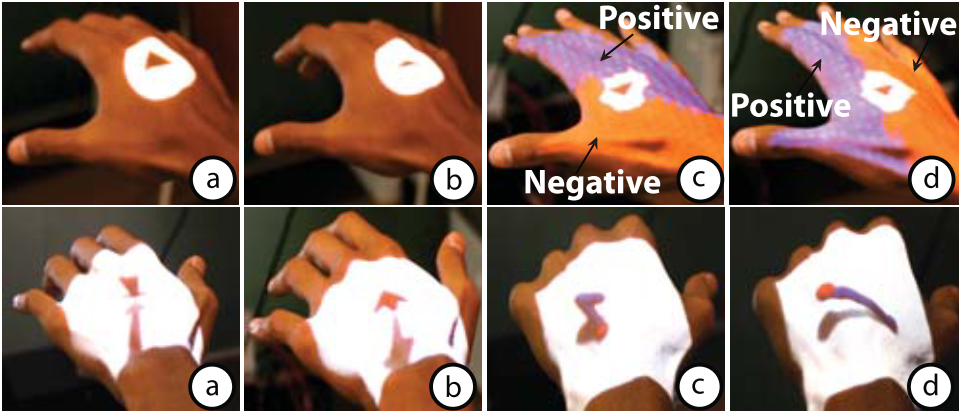
\includegraphics[width=\textwidth]{imgs/lightguide}
\centering
%\caption{LightGuide Visual Cues, extracted from the work of Sodhi \cite{Sodhi2012}.}
\label{fig:lightguide}
\end{figure}

\section{Tracking Techniques} 

Tracking devices have enabled the development of more immersive interactive applications.
Whether it be for entertainment or more serious matters, the possibility of interacting with 
an interface without using any kind of handheld devices can greatly enhance a user experience.

Nowadays it is possible to obtain affordable tracking devices such as Microsoft's Kinect, which 
can provide full skeleton tracking without the use of any kind of special equipment.
As opposed to more professional solutions that require special suits with markers, but provide a more accurate tracking. 
Even so, studies have shown that Kinect has an acceptable accuracy in comparison with other motion tracking alternatives 
and can be considered a valuable option for its low price and easy portability \cite{Scano2014,Chang2012a}.

To provide interactive content, the user's body must be detected and its position passed as input. This input normally consists of several tracking points which represent body joints. Their relative position between one another give us a representation of the user's current body posture, since each connection between two joints can be considered a bone as we can see in the 
Fig. \ref{fig:joints}.
In the Kinect's case, being a markerless tracking device, these joints are defined through software.

%Aiming at rehabilitation, a comparison between two skeletons might be required. For example, to know how different is the patient's current posture from the therapist's we would need to compare both skeletons. This comparison can be inaccurate if we take into account the existence of physical differences between them (arms with different lengths for example).\todo{Trabalhar melhor isto. Dizer explicitamente que o paciente deve ter que reproduzir os movimentos do terapeuta.} 

Aiming at rehabilitation, using tracking technology could enable applications to track a therapist's demonstration of a given movement prescribed to a patient.
Then, when the patient performed it, his movement could also be tracked and compared to the therapist's demonstration to detect possible errors.
For this to be possible, several factors have to be taken into account like the possible physical differences between both. If we were to make a ``blind`` comparison between both skeletons, the results would not be accurate.

Two comparison methods that can be used to address the aforementioned problem are described hereafter.

\subsection{Skeleton Comparison Methods}

In order to facilitate the description of the following methods, we will consider two given skeletons named SK1 and SK2, both with the same number of defined joints and where SK2 wants to mimic SK1's pose.

The first method of measuring differences between skeletons is through the usage of their joints position. 
As we can see in Fig.\ref{fig:sk1sk2}, SK1 and SK2's arms are not in identical positions. 
If we consider the euclidean distance between joints J11 and J12, they might never be considered equal if their arms have different lengths. 
If the euclidean distance never reaches zero, these two joints might never overlap. As we can see in Fig. \ref{fig:sk1sk2diff}, 
when both skeletons achieve identical pose, there still exist a distance \textit{A} between them, therefore by using the joint position 
this would not be an identical pose between them.
To solve this problem, another method must be used for comparison, 
which relies on other measurements not dependent of, i.e. invariant to, joint specific position. 

If we use the joint angles for comparison, it is possible to achieve better results due to 
the physical differences not influencing the measurements \cite{Borghese2013}. 
In this case, looking once more at Fig. \ref{fig:sk1sk2diff}, 
if we take into account the joint angle \textit{B}, both skeletons can be considered to have an identical posture, even though they have different arms length.

The accuracy of skeleton comparison has a important role in rehabilitation systems 
where the patient will be corrected in real-time. His body tracking data will be the 
base of the system behaviour and it will influence how it responds to the patient. 
Next, we will analyse the state of art concerning several different approaches for 
the provisioning of feedback information to the patient.

\begin{figure}[t!]
	\centering
	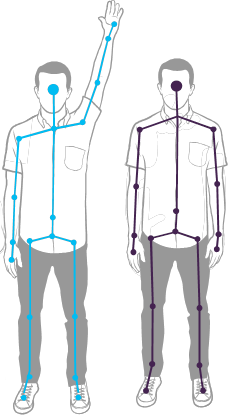
\includegraphics[scale=0.7]{imgs/joints.png}
	\caption{Joints position from Kinect}
	\label{fig:joints}
\end{figure}


\begin{figure}[t!]
	\centering
	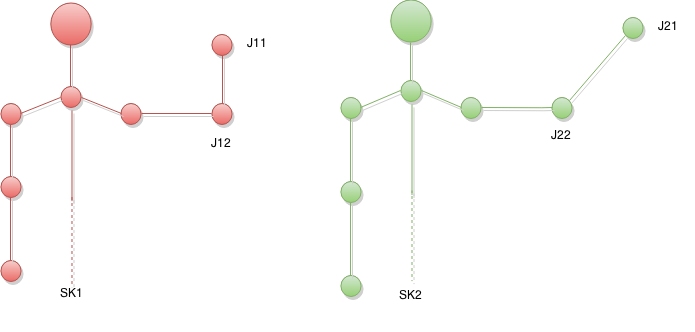
\includegraphics[scale=0.5]{imgs/SK1SK2.png}
	\caption{SK1 shows desired pose, SK2 midway to achieving it}
	\label{fig:sk1sk2}
\end{figure}

\begin{figure}[t!]
	\centering
	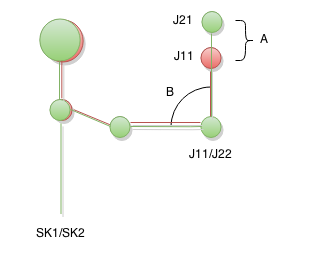
\includegraphics[scale=0.5]{imgs/sk1sk2diff.png}
	\caption{SK1 and SK2 overlapped}
	\label{fig:sk1sk2diff}
\end{figure}



\section{Information Feedback}
\label{RW-MF}

The basic goal of feedback is, as the name says, to feed information back to the user. 
It does not have to be in a textual form even though that is the most 
common form of feedback used for humans. We can receive information 
by using different means of communication. 
Everyday we are constantly processing information through a wide variety of ways like when 
we know someone is at the door because we hear the door ring bell or we recognize a friend within our sight.
Our senses are constantly at work to provide us information about our surroundings.
We can think about our senses as some sort of input sensor, each one designed for a specific type of information.

The information we receive from around us has an influence on our behaviour.
When a patient is attending physical therapy, the therapist is constantly interacting with him. 
This interaction is important in order for the patient to keep doing correctly the rehabilitation.
Not only does the therapist tells him what to do but also demonstrates it and, whenever necessary, physically corrects him.
What we observe here is the use of three different types of feedback being given to the patient - audio, visual and haptic,
each one being interpreted by hearing, sight and touch respectively.

For an automated rehabilitation system to successfully work, these interactions must 
be simulated by other sources of feedback, in a way that the patient understands 
what he must do without the presence of the therapist.

Visual feedback information is often used in rehabilitation systems to communicate with a user \cite{Design2005}. 
As one example of visual feedback on an \ac{AR} perspective, we have the overlaying of 
information on an interactive mirror for the user to analyze his performance in real-time \cite{Anderson,Tang2014a,Velloso2013,Klein2013,Alhamid2012a,blum2012}. 

Since there are multiple forms of giving feedback to a user, we can see examples where more than one are used at the same time.
Combining forms of feedback can provide better understanding of the tasks to a user by minimizing the amount of 
information given in a visual form and, instead, distribute it. 
But if not designed with caution, a system can end up overloading the user with too much information at the same time. 

\subsection{Feedback Applications}

A system that makes use of just one type of feedback is called a unimodal feedback system. 
In contrast, a system that is able to interact in more than one form of communication is considered a multimodal feedback system.
The main goal of using multimodal feedback is to provide a more complete interaction with the user, 
since different types of feedback can complement each other and enhance the user comprehension\cite{Sigrist2013}.

Alhamid et al. \cite{Alhamid2012a} proposed a system
that implemented an interface between a user and biofeedback sensors (sensors that are able 
to measure physiological functions). Even though it is not aimed for rehabilitation, his approach on user interaction can be analyzed.
Through this interface, the user was able to access data about his body and health thanks to the measurements made by the biofeedback sensors.
This system was prepared to interact with the user using multiple response interfaces, each one intended for specific purposes.

The visual interface relied on a projector that showed important messages and results from the biofeedback measurements.
In the other hand, the audio interface was responsible for playing different kinds of music through speakers. 
The music was selected depending on the user's current state. For example, if high levels of stress are detected, 
calming music would be played to help the user relax.

One of the most common approaches on visual feedback is the augmented reality mirror already discussed at section \ref{RW-AR}. Its common
use is justified by the fact that even without overlaying virtual images, it enables the user to have a spatial awareness of his own body.
But since a simple reflection does not provide guidance, we could observe several examples of augmented feedback being applied to the mirror.

Tang et al. \cite{Tang2014a} explored two different designs for visual guidance on a mirror aimed at upper-limbs movement.
Their first iteration consisted of virtual arrows that pointed at the targeted position for the user's hand.
The second provided a trace of tubes placed along a path which represented the complete movement to be performed by the user's arm.

In both cases it was detected some difficulty in depth perception. 
This kind of visual cues has proven not to be suitable for exercises 
where the user had to move his arm towards the camera or when he had to contract it.

Anderson et al. \cite{Anderson} tried to provide a more detailed visual feedback 
by using a full virtual skeleton placed over the user reflection. In this case the goal 
was to mimic the skeleton's pose and hold it for a specific time.
To diminish the lack of depth perception, a second tracker was placed on the user's side. 
Every time the system detected a large error on the z-axis, a window would appear with a 
side-view of both the virtual and user's skeleton for him to be corrected.

Unlike the above solution, LightGuide \cite{Sodhi2012} does not rely on interactive mirrors or screens to 
apply its visual feedback. By using a depth-sensor camera and a light projector, they were able 
to project information on the user's hand. This system was able to guide the hand through a defined 
movement by projecting visual cues. All the information projected on 
the hand was being updated in real-time influenced by the current position given by the tracking device.

The visual cues varied according to the desired direction of the movement. 
If the current movement only required back and forward motion, only one dimension was being used. 
Therefore, the visual cue would only inform the user where to move his 
hand in the z axis through a little arrow pointing to the correct position.
Two dimensional movements would combine the first visual cue by virtually painting the
remaining of the hand with a color pattern. The portion of the hand closer to the
desired position, would be painted with a different color than the remaining portion.
They concluded that by using LightGuide, most of the users could better execute a certain 
movement than if they were following video instructions.

Wellner et al. \cite{Wellner2007a} developed a study in which the use of sound feedback was tested in the rehabilitation
of stroke and spinal cord injured patients. They stated that audio feedback should not be used exclusively but it 
could be used as a complement of other feedback types.
The work environment involved a virtual scenario with a 3D human-shaped avatar that took a step every time the
patient took one too. The virtual scenario provided a visual feedback of what was happening in the simulation.
The patient was being held by an exoskeleton structure due to his inability to stand on his 
own, which also helped him taking steps by moving along with his legs. 

One of the challenges given to the patients was to walk in a virtual corridor where small obstacles would appear in front of the avatar. 
In addition to seeing the obstacle, audio feedback was also provided to help the user to cross it.

The audio feedback was used to inform the patient about two factors: the distance until 
the next obstacle and his foot current elevation. 
For the distance to the obstacle, a short beep sound was produced every time interval, which was influenced by 
the proximity of the obstacle, similar to the idea of a sonic radar which beeps faster as an object keeps getting closer. 
As for the foot elevation, a continuous 
sound was played during the challenge, while its pitch changed according to the elevation. 
This allowed them to test the same challenge with and without the audio feedback, to conclude if it could 
influence the overall performance of a patient. Haptic feedback was also used when a patient successfully crossed an obstacle.

Even though the use of sound feedback did not significantly improved overall results, a
slight confidence gain was detected on the user's performance while using it.

Focusing on the haptic feedback, Causo et al.\cite{Causo2011} presented a 
paper where vibration and visual cues were used for arm posture correction.
After selecting one from the six arm postures recorded, their goal 
was to successfully guide a patient to that same arm posture using the available feedback.

The haptic feedback could be originated from three different 
vibrating motors attached to the patient's arm, related to 
rotation on each of the three axis respectively (also known 
as \textit{yaw, pitch and roll}). Each one of this actuators 
could be independently activated in order to correct his arm 
posture within a single axis.

In their experiments, a comparison was made between using solely 
the haptic feedback and combining it with visual cues. 
The results shown that using only vibration, a subject 
could achieve the correct posture, even though he would 
take much more time achieving it in comparison to the time 
it took when using both visual and haptic feedback at the same time.
Therefore, even though haptic feedback could be used for guidance, its use 
could be more suitable for quick corrections and error augmentation to rapidly 
warn the patient of what is being wrongly done. 

\section{Related Work Overview}



After analyzing several examples of feedback approaches, it is possible to make some conclusions about their usefulness, whether it be rehabilitation-oriented or not.

Below, at the Table \ref{table-rw}, a summary of the state of 
the art can be found that provides a notion of which feedback types are the most used. 
Each work is also categorized accordingly to specific features. These categories, which describe some key features that each work may or may not have, are as follows:
\begin{itemize}
\item \emph{\textbf{Pa.}} - The \textbf{Pa}th required to execute the movement is taken into account, useful to prevent wrong executions of exercises.
\item \emph{\textbf{Ta.}} - The goal is to achieve a specific \textbf{Ta}rget. If path is not taken into account, any movement is valid as long as it reaches the target posture.
\item \emph{\textbf{R.T.}} - \textbf{R}eal \textbf{T}ime feedback is provided to keep the subject constantly informed about his performance.
\item \emph{\textbf{Gu.}} - Feedback given with the purpose of \textbf{Gu}iding the subject through a correct path. Helps the subject predict where to move. 
\item \emph{\textbf{Er.}} - Feedback given is based on subject \textbf{Er}ror. Constantly corrects the subject until goal is achieved
\item \emph{\textbf{S.G.}} - Use of \textbf{S}erious \textbf{G}ames, for movement encouragement. Not completely focused on guidance.
\end{itemize}

Indeed, each of the three types of feedback observed, namely visual, audio and haptic, have shown to be more suitable for different purposes.
Visual feedback appears to be normally used in regard to spatial information, due to the perception of space being the most precise when using the sense of sight. For this reason,
the best option to guide a patient through movements seems to be by using visual guidance.
But it is important to note that visual feedback still is a rather broad concept, therefore we could observe different takes on the whole subject of visual guidance.

The \ac{AR} mirror, discussed at section \ref{RW-mirrors}, is the most common 
solution to provide visual feedback, given that it can add information to the already present
mirror reflection. Even though a problem seems to persist throughout the several examples, namely the lack of depth perception.
But other approaches might have a chance of solving this problem if one tries to combine them both.

The use of projection mapping,might bring some improvements to visual feedback. 
Based on the \textit{LightGuide} from Sodhi et al. \cite{Sodhi2012}, there are reasons to be optimist 
about this possibility. With LightGuide, projection mapping was applied only to the hand, but their results 
are a good motivation to extend projection mapping to the full upper-limb and experiment with it.
This technique has been normally used for entertainment and, to our knowledge, has not been fully explored 
in a rehabilitation context. 

Unlike visual, audio and haptic feedback do not require the patient to keep his focus on the external feedback source. 
It allows him to concentrate on his own movement and receive feedback without looking at it, although it becomes 
more difficult to guide the user through more complex movements.

Audio feedback, even though being used in several of the described works, did not have such an important role as the visual feedback. 
Despite not normally being the main source of a patient's guidance, there is significant evidence that a rehabilitation system 
can benefit from using audio for some of its needs.
Sound does not only help with the immersion in a rehabilitation environment but it is also useful to alert the patient about specific events. It 
can provide the patient with a better control of his timing when necessary, for instance to inform him 
of the right moment to evade an obstacle \cite{Wellner2007a}. This application of audio feedback is backed 
up by the fact that the sense of hearing provides a great perception of temporal information \cite{Sigrist2013}.

%\begin{table}[t]
%\centering
%%\begin{tabular}{lccccccccc}
%\cline{2-10}
%\multicolumn{1}{c|}{} & \multicolumn{3}{c|}{Feedback Types} & \multicolumn{6}{c|}{Categories} \\ \hline
%\multicolumn{1}{c}{Authors} & Visual & Audio & Haptic & Pa. & Ta. & R.T. & Gui. & Err. & S.G. \\ \hline
%Anderson et al.\cite{Anderson} & \ding{51} & \ding{51} &  & \ding{51} &  & \ding{51} & \ding{51} & \ding{51} &  \\ \hline
%Borghese et al.\cite{Borghese2012,Borghese2013} & \ding{51} & \ding{51} &  &  &  & \ding{51} &  &  & \ding{51} \\ \hline
%Burke et al.\cite{Burke2009} & \ding{51} & \ding{51} &  &  & \ding{51} & \ding{51} &  &  & \ding{51} \\ \hline
%%Gama et al.\cite{Gama2012a} & \ding{51} &  &  &  & \ding{51} & \ding{51} & \ding{51} & \ding{51} &  \\ \hline
%Klein et al.\cite{Klein2013} & \ding{51} &  &  &  & \ding{51} & \ding{51} &  &  &  \\ \hline
%%Sadihov et al.\cite{Sadihov2013} & \ding{51} &  & \ding{51} & \ding{51} &  & \ding{51} & \ding{51} &  & \ding{51} \\ \hline
%Schonauer et al.\cite{Schonauer2011a,Schonauer2011c} & \ding{51} &  &  &  &  & \ding{51} &  &  & \ding{51} \\ \hline
%Sodhi et al.\cite{Sodhi2012} & \ding{51} & \ding{51} &  & \ding{51} &  & \ding{51} & \ding{51} &  &  \\ \hline
%Tang et al.\cite{Tang2014a} & \ding{51} &  &  & \ding{51} &  & \ding{51} & \ding{51} &  &  \\ \hline
%Velloso et al.\cite{Velloso2013} & \ding{51} &  &  & \ding{51} &  & \ding{51} & \ding{51} &  &  \\ \hline
%Wellner et al.\cite{Wellner2007a} & \ding{51} & \ding{51} & \ding{51} &  & \ding{51} & \ding{51} &  & \ding{51} & \ding{51} \\ \hline
%\end{tabular}
%\caption{Summary of feedback used in state of art and categories}
%\label{table-rw}
%\end{table}

Observing the Table \ref{table-rw}, we can see that haptic feedback was 
the least used of the three. Perhaps due to requiring more specialized equipment to apply more 
detailed feedback, unlike audio which requires only a set of speakers and visual which can be 
achieved just as easily. Even so, haptic feedback could be useful to emphasize certain aspects, 
such as error augmentation \cite{Causo2011} which may promote motor learning due to enabling a 
patient to be more aware of his mistakes\cite{Sigrist2013}.
For haptic feedback to be used for guidance purposes, it would be necessary to have equipment 
capable of applying physical force on the patient, but since visual feedback has already proven 
to be an adequate provider of spatial information, we can place haptic feedback in a secondary 
position.
 
 

\chapter{SleeveAR}
\label{sec:sleevear}

\section*{Summary}

Before implementing SleeveAR, it was vital to fully establish what were our goals and what we wanted to achieve. 
The following chapter describes our vision of this work and lists the features we considered to be a minimum requirement for a successful implementation.



\section{Vision}

SleeveAR aims further beyond the accomplishments LightGuide was able to make. 
As described in the previous section, LightGuide only focused on projecting information on top of the hand. Not only does this leave a small room for movement variety, but also the amount of possible information given can be quite reduced.
By increasing the projection area throughout the whole arm we can successfully improve an user's awareness while an movement is being executed. 
Not only that, but if it was possible for the movement being replicated to be originated by another person, we could achieve much more realistic and useful guidance.
With SleeveAR virtual content can be projected onto different surfaces, and even, onto people's own limbs, to provide, in real-time, a more immerse experience. 

Our vision consists on two main concepts. Firstly, the precise recording of the exercise being demonstrated by a personal therapist. 
And secondly, the ability to properly guide another person, the rehabilitation subject, during the execution of the pre-recorded exercise.
Next we will describe in detail each of this general concepts of our vision.

%While, at the same time, provide awareness of the rehabilitation exercise progress to insure the correctness of the patient's movements.
%With SleeveAR, a therapist can easily demonstrate the prescribed exercises and make sure his patient will perform them correctly without the requirement of his close supervision.

%In the SleeveAR system, the exercise being performed needs to be recorded beforehand, which, in this case, should be a health professional. 
%Not only it provides a great range of possible movements, but also assigns,onto the professional, the responsibility of providing adequate exercises based on a specific patient's condition.

\section{Recording}

Normally, when a patient executes prescribed exercises, these same exercises were specifically made for the current patient's condition. 
With this in mind, we wanted to maintain that relation between a therapist and patient. 
To do this, we chose to give the therapists the power of demonstrating the exercise they want the patient to do. 
Based on this demonstration, SleeveAr will capture the therapist movement and store it for later use.
By giving the therapist the responsibility of demonstrating the exercise, we do not need to worry about the physical limitations of the patient that would use our system to recreate it. 
We are assuming the recorded exercise is already customized for the patient in question.

Given these assumptions, SleeveAr must then be able to guide a patient through those exercises as best as it can. Next we describe the behaviour SleeveAR should have while guiding a patient.


\section{Guiding}

Guiding a patient through an exercise can be divided in three phases in our approach, which are as follows:

\begin{itemize}
\item Reaching Initial Position
\item Performing Exercise
\item Performance Review
\end{itemize}

We consider these three phases to be a simple and clear way of organizing what SleeveAR should do when interaction with an patient. Next we describe each of them.

To successfully recreate an exercise, we considered the user must first reach the exercise initial position, i.e., the first arm position from the recorded demonstration.
To do this, a patient must follow SleeveAR's feedback in order to achieve the correct arm position. 
All feedback used for this first phase is explained in section \ref{vision-feedback}.
After SleeveAR considers the initial position has been reached, we can now start guiding the user through the remaining exercise.

It could be an almost impossible task for a patient to recreate an exercise exactly the same as the original. 
With this in mind, SleeveAR needs to rely on thresholds for specific values. 
By doing so, if it was required of a patient to achieve, for example, a 90 degree arm flexion, he would not 
need to actually achieve it, being only enough for him to get close to that degree of flexion.

Finally at the end of each exercise, SleeveAR should provide an overview of the patient's performance in comparison with the original. 
This will help the patient understand what he might have done wrong and in which parts of the exercise he could still perform better.

To successfully guide a patient through his exercises while informing him of his performance, we need to plan how will SleeveAR interact with its users. 
Next section will describe our planned designs for providing real-time and interactive feedback aimed at the user.

\section{Visual Feedback}
\label{vision-feedback}

\begin{figure}[!t]
    \begin{center}
        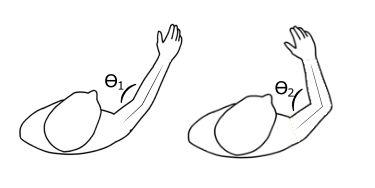
\includegraphics[width=0.5\textwidth]{imgs/elbowangle.png}
    \end{center}
    \caption{Definition of the elbow angle.}
    \label{fig:elbowangle}
\end{figure}

Providing useful and minimalist design was our goal when designing our visual feedback. There were some key points we wanted to address when designing it.
First of all, the visual information had to provide the user with a representation of his \textbf{current} position, while also showing the \textbf{desired} position. 
These representations had to be done in a way the user would easily comprehend what to do in order to achieve that same desired position.
To provide suitable feedback regarding the full arm we first applied different design for each of the regions. Next we will present our planned visual feedback designs.

\subsection{Fore Arm}

Before creating the fore arm visual feedback it was important to understand what type of movement could be executed with this arm region.
The fore arm is connected to the upper arm by the elbow joint and its range of motion could be summarized in extension and flexing of the arm.
When extending or flexing the arm, we basically are changing the elbow angle, given by the angle between the upper and fore arm.
If we look at figure \ref{fig:elbowangle} we can see an example of two different elbow angles. On the left, we see an elbow angle $\theta$$_1$ of approximately 180 degrees, while on the right an elbow angle $\theta$$_2$ of 90 degrees.  

As we said previously, we wanted both designs to represent the current and desired state. Our final design for a fore arm feedback makes use of a circle with two bars, similar to a clock with two pointers.

%\subsubsection{Current State}

\begin{figure}[!t]
    \begin{center}
        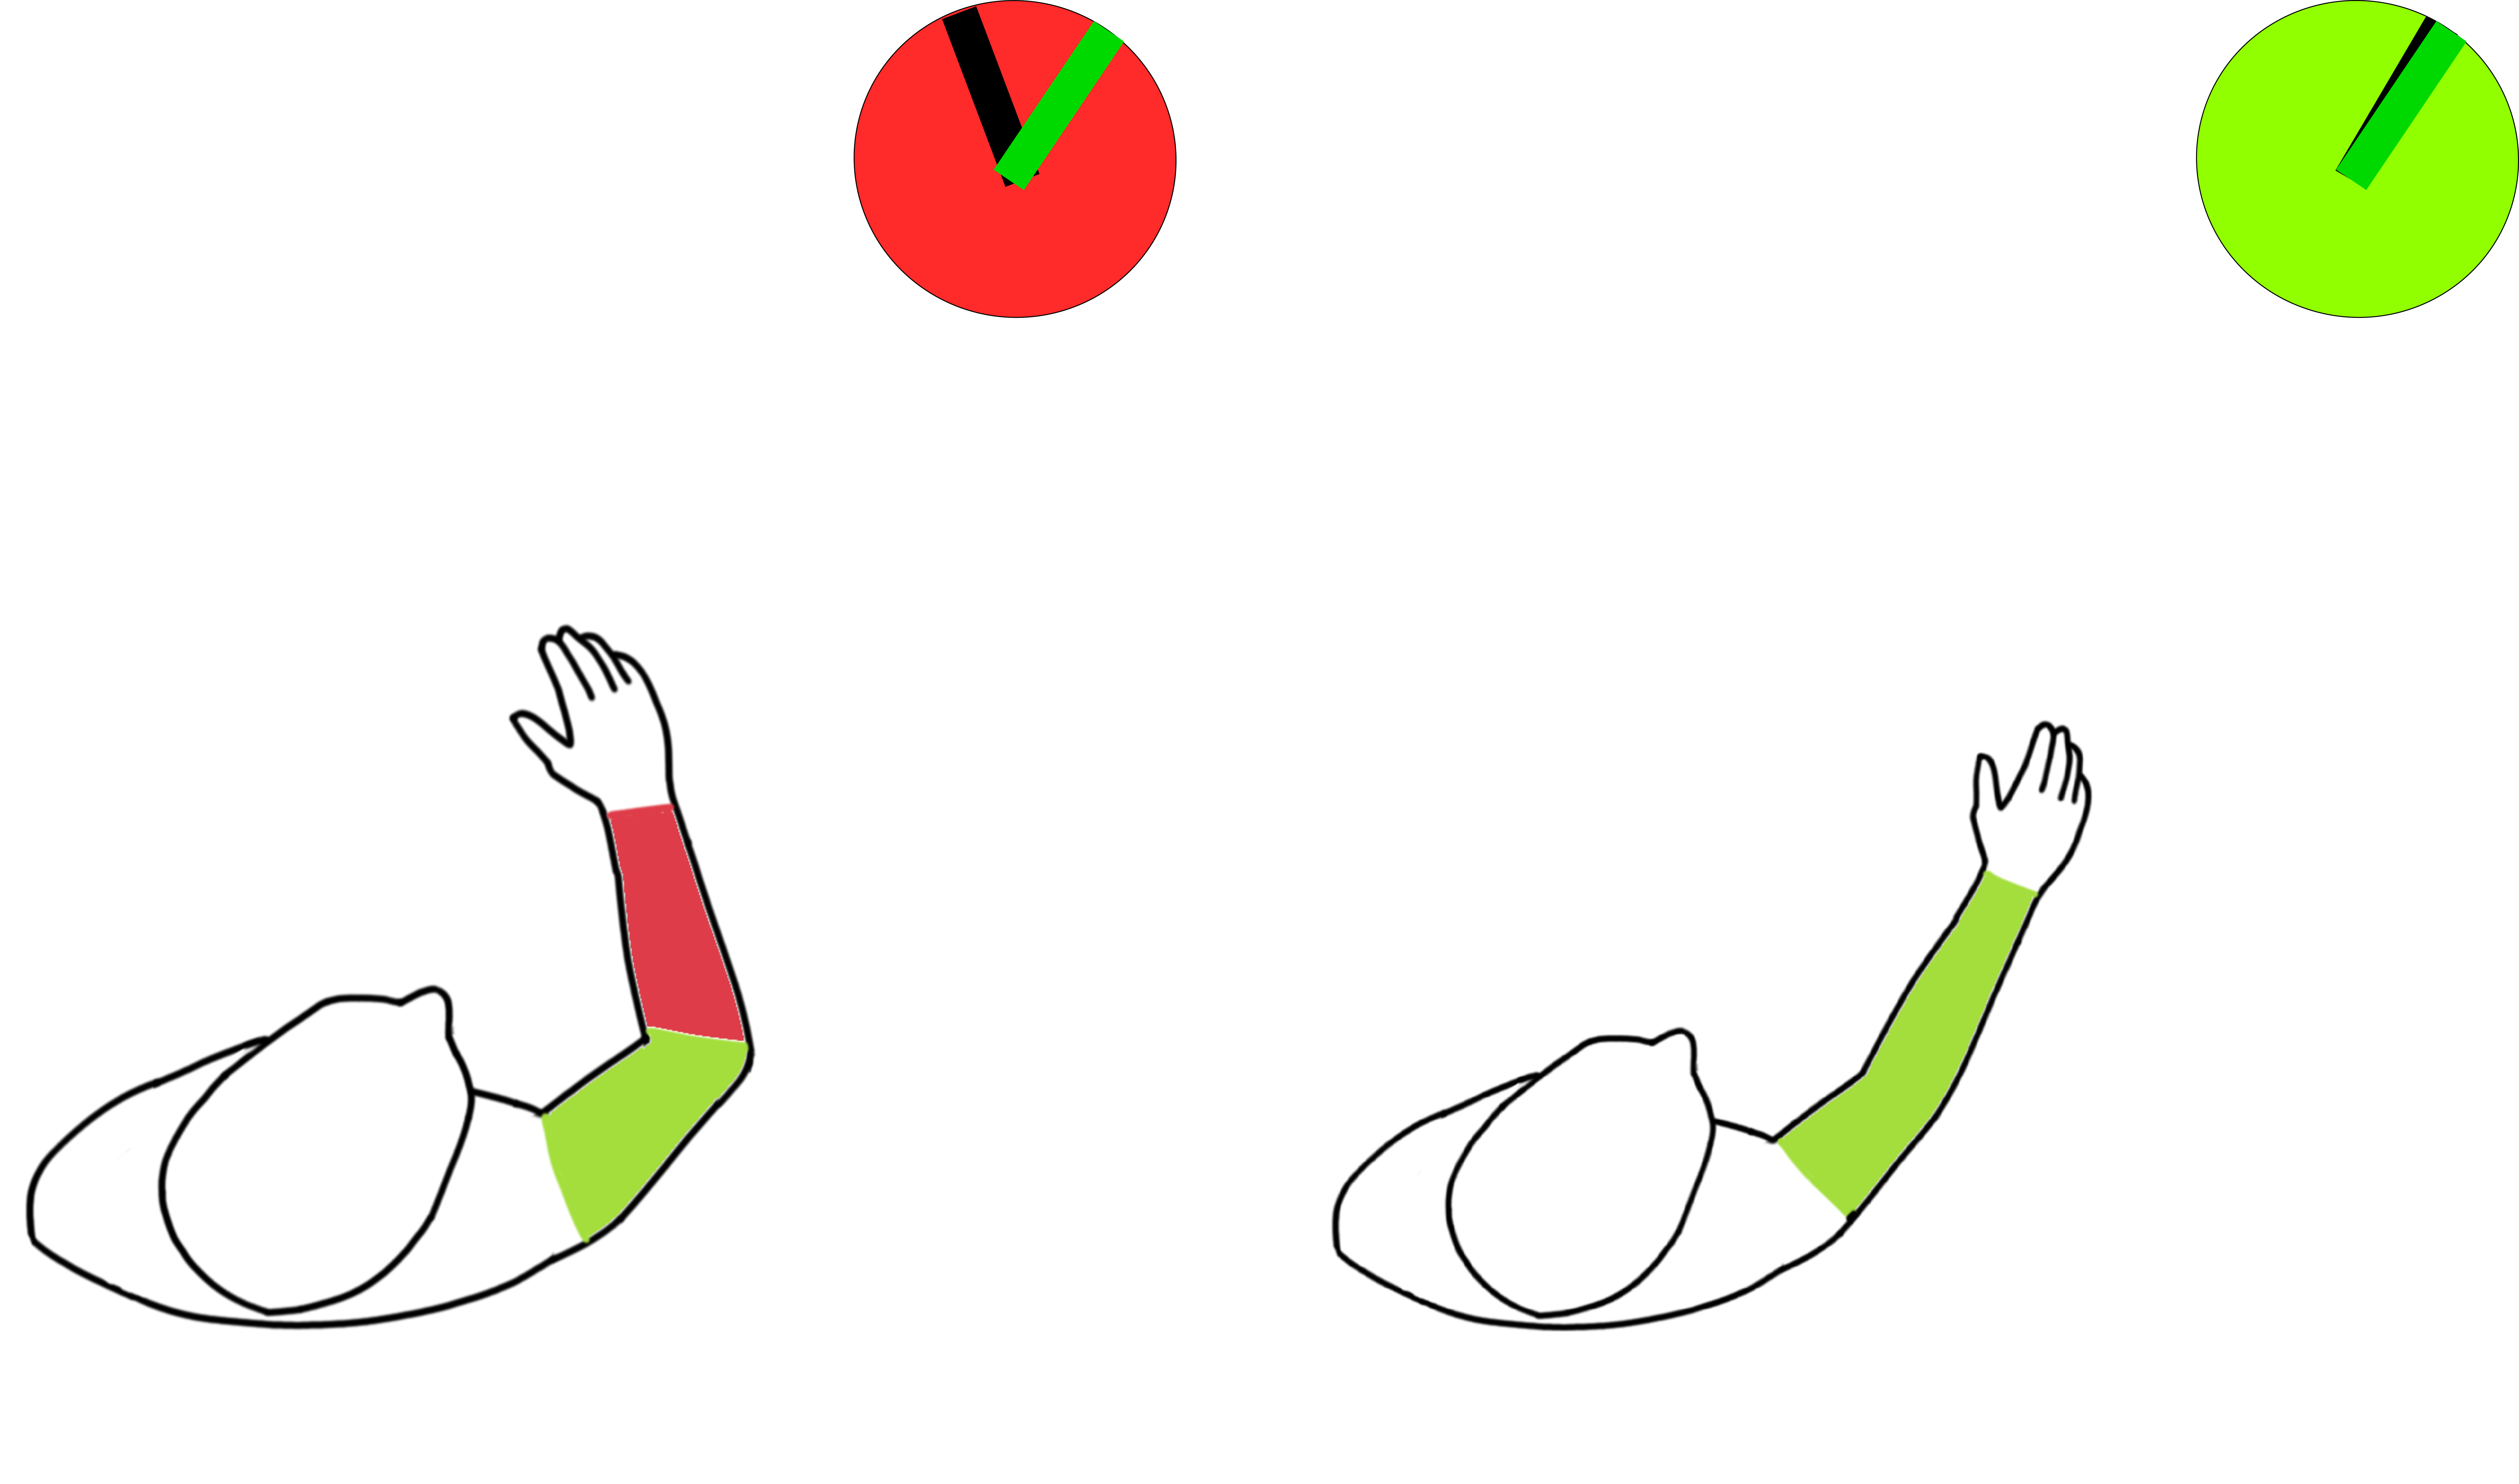
\includegraphics[width=0.5\textwidth]{imgs/forearmfeedback.png}
    \end{center}
    \caption{Visual Feedback based on fore arm.}
    \label{fig:forearmfeedback}
\end{figure}

To represent the current state, we use the black bar, seen in figure \ref{fig:forearmfeedback}. Whenever the user moves his fore arm, this bar will move accordingly.

%\subsubsection{Desired State}

The desired fore arm state is represented by the green bar. For the user to achieve this state, is is required of him to move his fore arm in order for the black bar to reach the green bar.

%\subsubsection{Additional Information}

To extend the user's awareness we added two additional features specifically to this design. Depending on the distance between both bars, the circle color would fade between red, too far, and green, close enough. Also, if the black bar gets too far from the desired position, rotating arrows will appear to wan the user he is currently not correctly positioned. Next we present the planned design for the upper arm feedback.


\subsection{Upper Arm}

\begin{figure}[!t]
    \begin{center}
        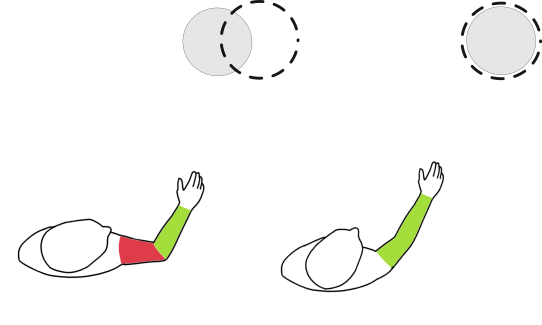
\includegraphics[width=0.5\textwidth]{imgs/upperarmfeedback.png}
    \end{center}
    \caption{Visual Feedback based on upper arm.}
    \label{fig:upperarmfeedback}
\end{figure}

As for the upper arm region, the type of movement allowed can be represented by the direction it is pointing to, which is obtained by a direction vector from the shoulder to the elbow as seen in fig \todo{figura}.
Once again, it was necessary for the design, seen at fig \ref{fig:upperarmfeedback} to both show the current and desired state. 

%\subsubsection{Current State}

To represent the upper arm current direction, a dotted circumference was chosen. By moving the upper arm vertically or horizontally, the dotted circumference should move, respectively, vertically and horizontally.

%\subsubsection{Desired State}

As for the desired state, a simple circle was chosen. For the upper arm to achieve the desired direction the user simply has to move it until the dotted circumference surrounds the circle.

\subsection{Full Arm}

\begin{figure}[!b]
    \begin{center}
        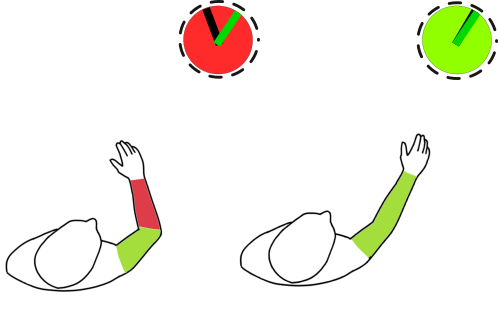
\includegraphics[width=0.4\textwidth]{imgs/fullarmfeedback.png}
    \end{center}
    \caption{Combination of both visual feedback designs.}
    \label{fig:fullarmfeedback}
\end{figure}

Each one of the previously presented designs are able to guide each arm region individually.
In order to guide a user to a full arm position, we combined both of them as seen on fig \ref{fig:fullarmfeedback}.

By replacing the grey circle, used on the upper arm's design, with the elbow angle circle from the fore arm's design, we are able to use both of them simultaneously. 

All these designs are able to guide the user to a specific, but static, position. For us to be able to guide a user throughout a movement, there need to be some changes on it.

In addition to the already presented feedback, which will be projected on the floor, we will also project information on top of the user's arm. 
In this case, we will not provide feedback as detailed as it is being provided on the floor. 
Instead, we will project diferent colors in each arm region depending on how far they are from the desired state. 
Once again, looking at figure \ref{fig:armvisualfeedback} we can observe the 
different arm regions having different colours on top, depending on the user's arm position.
These arm color projections will help in highlighting what the user might be doing incorrectly whiteout losing focus on the main feedback.

\subsection{Movement Guidance}

During an arm movement, we can not assume that both the upper and fore arm will remain the same. We can have an example were the arm remains fully extended throughout the movement or where the fore arm varies during the movement. In this case there's an elbow angle variation which mean the fore arm desired state is continuously changing.
With this in mind, our planned feedback must then change its desired state during the movement.

As for the upper arm, to help the user know to where he must move it, a path will be drawn showing the direction to where he must go. If we look closely at the previously presented design, we can observe it actually focus around the circle. The fore arm changes the circle itself, while the upper arm controls the dotted circumference that must cover also the circle. With this in mind, if we move this same circle through the movement path, we will be able to continuously inform the user about the desired direction while also updating what specific elbow angle he should have. In fig \ref{fig:movementguidancefeedback} we can see an example of this, where the user is already midpoint in the exercise.



\begin{figure*}[!t]
    \begin{center}
        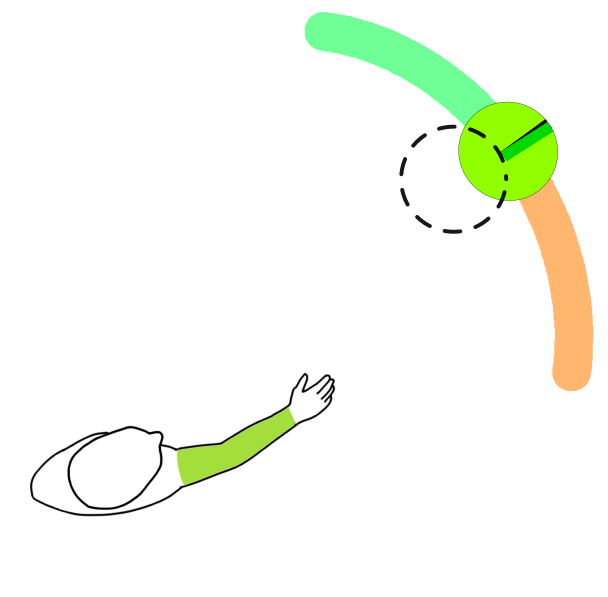
\includegraphics[width=0.4\textwidth]{imgs/movementguidancefeedback.png}
    \end{center}
    \caption{Visual Feedback during a movement.}
    \label{fig:movementguidancefeedback}
\end{figure*}


%Hereafter, as depicted in Figure~\ref{fig:vision}, 
%the patient follows all provided feedback to replicate the pre-recorded movement step-by-step, without ever seeing the exercise executed before.
%The current position of the subject's arm is being constantly tracked in order to always provide real-time 
%feedback based on how he should move it from that point.
%Visual feedback is achieved by projecting light onto his full arm and surroundings. The projection on the arm will enable us to 
%guide a subject through translations and rotations, using different kinds of visual cues to different situations. As for the projection on the subject's surrounding 
%will serve the purpose of providing other useful information not directly connected to the movement itself. 
%In Figure~\ref{fig:vision} we can observe a progress bar being projected on the floor. 
%This bar not only provides the subject an understanding of how far in the exercise he is at the moment, but also helps the subject visualize the angle of movement he should be doing.
%Audio and haptic feedback can help inform the subject about specific information, without making him loose his focus on the visual feedback.
%The haptic feedback is used to quickly notify the subject of any vital information about the current state of the exercise. 
%Awareness of erroneous movements is achieved mainly by the employment of vibration cues into the patient's arm.
%Furthermore, for the purpose of timing, auditory feedback provide the subject with information regarding when to start or stop the exercise by using recognizable audio cues %which represent those same actions.

%Interactive phases(Figure~\ref{fig:interaction}):
%\begin{itemize}
%\item {\bf Initial Position Phase:}
%\item {\bf Task Performance:}
%\item {\bf Progress Report:}
%\end{itemize}



\begin{figure}[!b]
    \begin{center}
        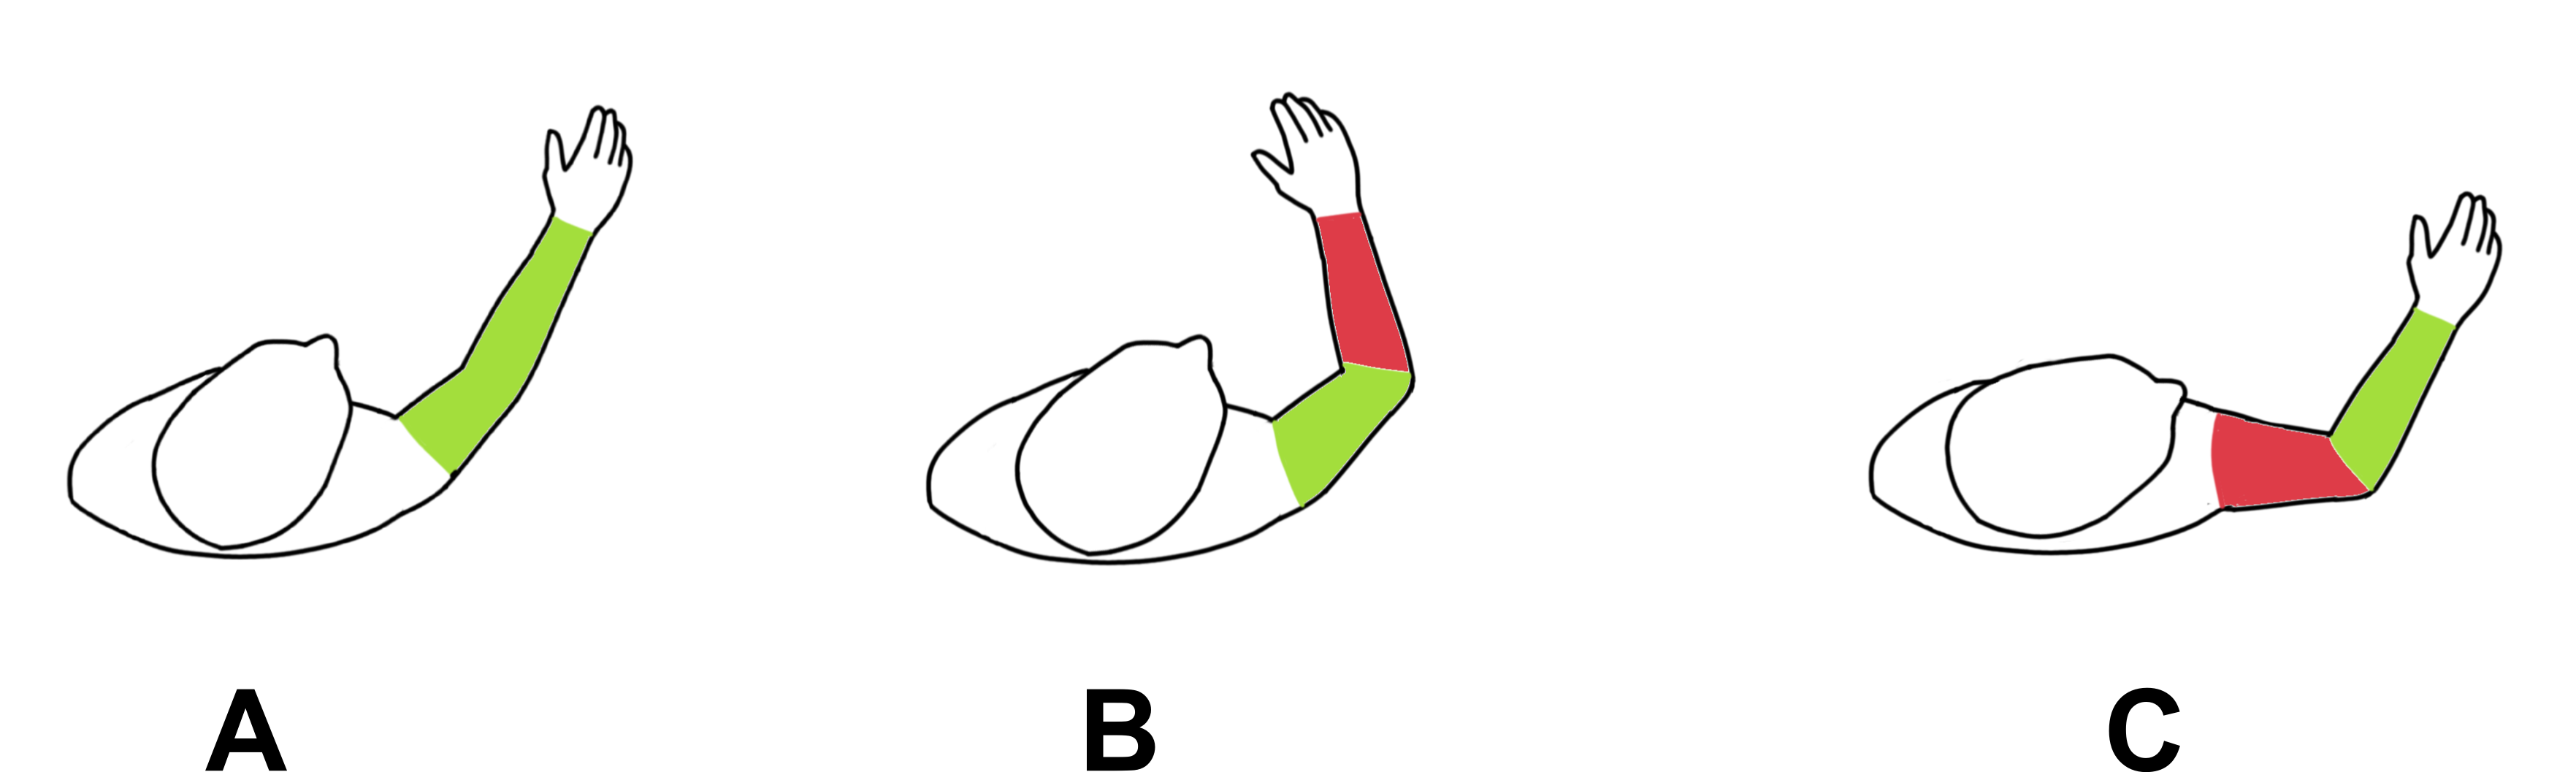
\includegraphics[width=\columnwidth]{imgs/armvisualfeedback.png}
    \end{center}
    \caption{Sleeve Projected Feedback: A) Correct Arm. B) Incorrect Fore Arm. C) Incorrect UpperArm}
    \label{fig:vision}
\end{figure}

\subsection{Performance Review}
%%%%%%%%%%%%%%%%%%%%%%%%%%%%%%%%%%%%%%%%%%%%%%%%%%%%%%%%%%%%%%%%%%%%%%%%%%%%%%%%%%%%%%%%%%%%
%                               My System 24pp
%%%%%%%%%%%%%%%%%%%%%%%%%%%%%%%%%%%%%%%%%%%%%%%%%%%%%%%%%%%%%%%%%%%%%%%%%%%%%%%%%%%%%%%%%%%
\chapter{Architecture}
\label{sec:Architecture}
 
\section*{Summary}
 
In this section, we will present our proposal which will be divided as follows. 
In the first place, in section \ref{section-approach-main-objectives} we explain
our goals in detail and what we consider to be an innovation. 
Next, section \ref{section-approach-architecture} will present the planned architecture with a step-by-step 
explanation for the reader to fully understand the desired work flow.
The final section will list the tools that we plan to use in the implementation of our approach.

\subsection{Main Objectives}
\label{section-approach-main-objectives}

Hereby, we present our proposal in which we aim to further explore the possibilities of multimodal 
feedback applied in a rehabilitation context.

We plan to combine multiple sources of feedback: visual, audio and haptic feedback, 
in order to evaluate how the patient responds to these sources of 
guidance throughout the execution of a given movement. 

To provide a dynamic feedback that constantly reacts to the patient's movements, we will rely on real-time skeleton tracking through a motion capture device.

The use of projection mapping in a rehabilitation environment has not been experimented yet, 
and we have reasons to believe it can bring great benefits to the methods of guidance 
applied to a patient in this kind of rehabilitation systems. If combined with an augmented reality mirror 
and audio or haptic feedback, we will be able to approach the same exercises in different ways in order to evaluate which 
feedback combinations can make the patient understand more clearly the required movements.

To control these feedback sources, a rehabilitation system will be implemented.%\todo{dar nome ao sistema?} 
The system will be capable of manipulating the feedback in order to guide
the patient through a predefined exercise which must be previously learned by the system through demonstration.
This way, the system is only responsible for guiding the patient to a correct execution of the chosen exercise.

We will focus this initial proposal only on exercises related to upper limb movement to simplify the implementation and reduce the number of factors that would need to be taken into account. This way we can experiment more with multimodal feedback and achieve more precise results.


\subsection{Architecture}
\label{section-approach-architecture}

The planned architecture of our proposal is divided into two different parts. 
The first, called \emph{Learning Architecture}, consists of the process for obtaining an exercise model by demonstration for further use.
The second and most important part, called \emph{Teaching Architecture}, concerns the application of the multimodal feedback for another person to recreate the exercise model.


\subsubsection{Learning Architecture}

The first part of our architecture serves the purpose of generating an exercise model which will be used for teaching and guiding exercises' execution.

As we can see in Fig. \ref{fig:learning}, we start by having a \ac{PT} demonstrating the prescribed exercise (1). Through motion capture devices, the \ac{PT} body is tracked during the demonstration and the tracking data is stored in a storage infrastructure.

Then, all the tracking data recorded is sent to the \emph{Exercise Generator Module} (2) in which the data will be sanitized (e.g., remove tracking data whenever the \ac{PT} is not performing the exercise) to be fed into the next step.

Finally, the resulting data will be returned from the \emph{Exercise Generator Module} to an element denoted \emph{Exercise Model} (3), which will consist of modelling all the useful data required to recreate the exercise initially demonstrated by the therapist. 

The generated \emph{Exercise Model} will be the foundation of our Architecture's second part, described hereafter.


\begin{figure}
	\centering
	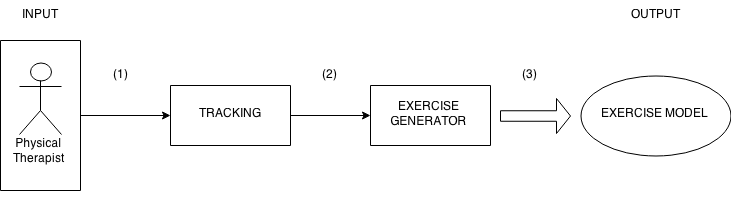
\includegraphics[width=0.8\textwidth]{imgs/LearningPhase}
	\caption{Learning Architecture Diagram}
	\label{fig:learning}
\end{figure}

%\caption{Learning Phase}
\subsubsection{Teaching Architecture}

The second part of our architecture serves the purpose of taking advantage of 
multiple feedback interfaces in order to guide a patient through 
the execution of a previously recorded exercise, the already described \emph{Exercise Model}.

As shown in Fig. \ref{fig:teaching}, it starts by 
loading the desired exercise that was generated in the \emph{Learning Architecture} (4), which will be the basis for comparison with the patient's body.

In this case, the tracking module is responsible for constantly sending the tracking data to the \emph{Multimodal Feedback Manager Module}(MFM) (5,6).

The \ac{MFM} module holds the core of our approach. While receiving real-time tracking data from the patient, the module will compare his current posture to the \emph{Exercise Model}.
With this in mind, the module will communicate (7) with the available feedback interfaces in order to guide the patient, for him to achieve a similar movement to the one recorded.
The module will manipulate each interface independently from one another, to easily create different combinations of feedback so that we can evaluate their validity.
Each one of the three feedback modules available will consist of devices capable of interacting in the desired feedback type: visual, audio or haptic. 

While the patient is still executing the exercise, the required feedback will continue to be applied (8, 9, 10). Therefore, as the patient keeps changing his posture, the tracking data will also be updated and therefore, affecting the resulted feedback.
This process (5-10) will remain in cycle until the given exercise is finished.


\begin{figure}
	\centering
	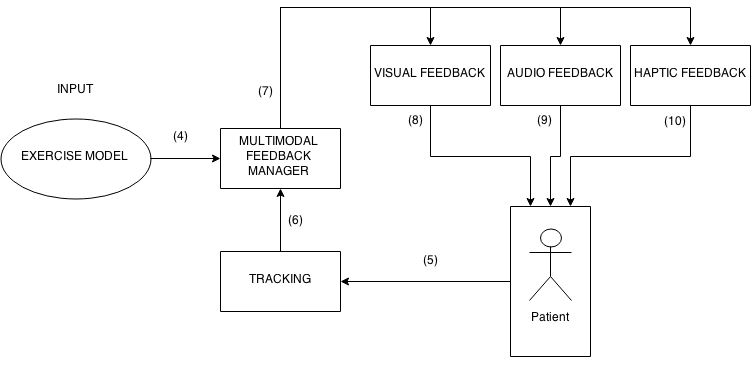
\includegraphics[width=0.7\textwidth]{imgs/TeachingPhase}
	\caption{Teaching Architecture Diagram}
	\label{fig:teaching}
\end{figure}
%%%%%%%%%%%%%%%%%%%%%%%%%%%%%%%%%%%%%%%%%%%%%%%%%%%%%%%%%%%%%%%%%%%%%%%%%%%%%%%%%%%%%%%%%%%
%                               My System 24pp
%%%%%%%%%%%%%%%%%%%%%%%%%%%%%%%%%%%%%%%%%%%%%%%%%%%%%%%%%%%%%%%%%%%%%%%%%%%%%%%%%%%%%%%%%%%
\chapter{Implementation}
\label{sec:implementation}

\section*{Summary}
%In this section, the hardware required to implemented our approach will be described. Even though some devices are still not certain, we present the possible alternatives to prevent that. In addition to the hardware, the software tools required will also be described. 

This section will describe the necessary steps taken for our SleeveAR's implementation. 
First of all, section \ref{sec:impl:arch} will briefly explain the overall architecture which served as a guiding tool for our implementation. 
Second, at section \ref{sec:impl:dev} we will dig deeper into the the most important aspects that made possible to develop the tool here presented.

\section{Architecture}
\label{sec:impl:arch}


\section{Development}
\label{sec:impl:dev}




\subsection{Tracking Devices}

For the proposed approach to work, it is necessary to track the subjects as accurately as possible. There are more than one available alternatives that can be used as the tracking device.

The first makes use of the recently released, Microsoft Kinect One\footnote{\url{http://www.xbox.com/xboxone/kinect}} 
(previously baptized as Kinect 2), which supposedly offers a better tracking quality than 
the previous version, Kinect 1. Although this might be true, to the best of our knowledge there are still no published studies which use the new Kinect in order for us to understand if this would be the best choice for our approach.

The other alternative available at our laboratories is an OptiTrack Motion Capture system \footnote{\url{https://www.naturalpoint.com/optitrack/}}. 
This option could offer us a more precise tracking and the possibility of dealing with occlusions due to the multiple cameras scattered around the room. The downside is the fact that 
it requires body markers to be used in order to successfully detect a person, unlike the 
Kinect which detects the human body through software algorithms.

Occlusion problems are much more likely to occur using Kinect than with the OptiTrack, due to only using one motion capture sensor. There can be moments where the patient could point his arms forward making the Kinect lose sight of the rest of the body. These problems were known to happen with the first Kinect, for the newest version we will need to understand if it still happens.

We intend to develop a comparison test between the tracking devices available. With this test we will be able to evaluate the tracking quality of each device and therefore decide which one would be the more suitable for our implementation. 

\subsection{Feedback Devices}

To be able to provide guiding cues to a patient, we will need a group of devices capable of providing each of the three possible feedback types that were presented.

For the visual feedback, we will rely on two concepts: the \ac{AR} mirror and projection mapping. 
For the first, we will capture the patient's image with a camera and project it into a screen. 
This way it is simulated a mirror, similar to other approaches discussed in this work.
As for the projection mapping, a light-projector will be used in order to, combining with 
the the tracking device, project visual cues on the patient's body.

To provide audio feedback, a set of speakers will be required around the patient. 
Therefore, enabling the reproduction of surround sound to explore possible sound localization experiments.

Finally, the haptic feedback will rely on vibration applied onto the user by using 
vibratory actuators attached to his arm. 
One possible option would be using the \textit{Pebble Smart watch}\footnote{\url{https://getpebble.com/}} that 
provides a Developer Kit to access its features, which includes vibration motors. 
By implementing a communication channel with the watch, it will be possible to control its vibrations whenever necessary.

\subsection{Software Tools}

To implement our software responsible for interacting with the several feedback interfaces that 
will be used, we will choose the \emph{Unity3D} game engine\footnote{\url{http://www.unity3d.com}}. 
This engine already provides several tools that facilitate the development of augmented reality applications and we have in our possession already developed frameworks to communicate with the available tracking devices.

The Kinect Tracking Device already provides an SDK for Unity applications which, if Kinect ends up the chosen tracking device, will accelerate the implementation of the Tracking Module described in section \ref{section-approach-architecture}.

As for the Pebble Smart watch, although there is an SDK available, it does not support Windows at the moment. If the Windows SDK is not released in the next weeks, we will use the other alternatives provided by the Pebble team which will consist on using an Android phone as a bridge between the Pebble and our application.
%%%%%%%%%%%%%%%%%%%%%%%%%%%%%%%%%%%%%%%%%%%%%%%%%%%%%%%%%%%%%%%%%%%%%%%%%%%%%%%%%%%%%%%%%%%
%                               Evaluation - 16pp
%%%%%%%%%%%%%%%%%%%%%%%%%%%%%%%%%%%%%%%%%%%%%%%%%%%%%%%%%%%%%%%%%%%%%%%%%%%%%%%%%%%%%%%%%%%
\chapter{Evaluation}
\label{sec:evaluation}

\section*{Summary}


\section{Methodology}

\section{Test Environment and Subjects}

\section{Results Analysis}

\section{Validation with Physical Therapist}
%%%%%%%%%%%%%%%%%%%%%%%%%%%%%%%%%%%%%%%%%%%%%%%%%%%%%%%%%%%%%%%%%%%%%%%%%%%%%%%%%%%%%%%%%%%
%                               Conclusions - 2pp
%%%%%%%%%%%%%%%%%%%%%%%%%%%%%%%%%%%%%%%%%%%%%%%%%%%%%%%%%%%%%%%%%%%%%%%%%%%%%%%%%%%%%%%%%%%
\chapter{Conclusions}
\label{sec:conclusions}

\section*{Summary}

\section{Conclusions}
Using augmented reality with multimodal feedback for rehabilitation allows a 
patient to have a source of guidance and correction when executing 
exercises outside of a clinic. This would be preferred, as opposed to exercising with no feedback where there is no way of correcting the execution.

\todo{THE TEXT BELOW IS RELATED TO MULTIMODAL - for future work. CHANGE to discuss the innovation brought by the solution, its advantages and disadvantages}

The state of the art presents several solutions to provide guidance during movement's execution, some already applying multimodal feedback. 
Even so, several problems with the patient's perception of the feedback have been reported, and clearly there is still room for improvement when combining sources of feedback.

With our proposal, we will be able to evaluate which feedback 
combinations could be more suitable for guiding a patient while solving some of the perception problems and also 
contribute with different feedback techniques in addition to the ones observed in the state of the art.

\section{Future Work}

As future work we would like bla bla.

\todo{improvements as reffered by therapist, testing on a real therapeutic environment with real patients, extending to account for multimodal feedback, etc}


\bibliographystyle{ieeetr}
\bibliography{references}
\addcontentsline{toc}{chapter}{{\small Bibliography}}


\end{document}
